\newpage
\section{$NO_x$ process model derivation from governing equations}
The discrete nonlinear recursive model that is linear in parameters can be derived from the molar conservation equations directly. The model derivation involves three main steps:
\begin{figure}[H]
        \centering
        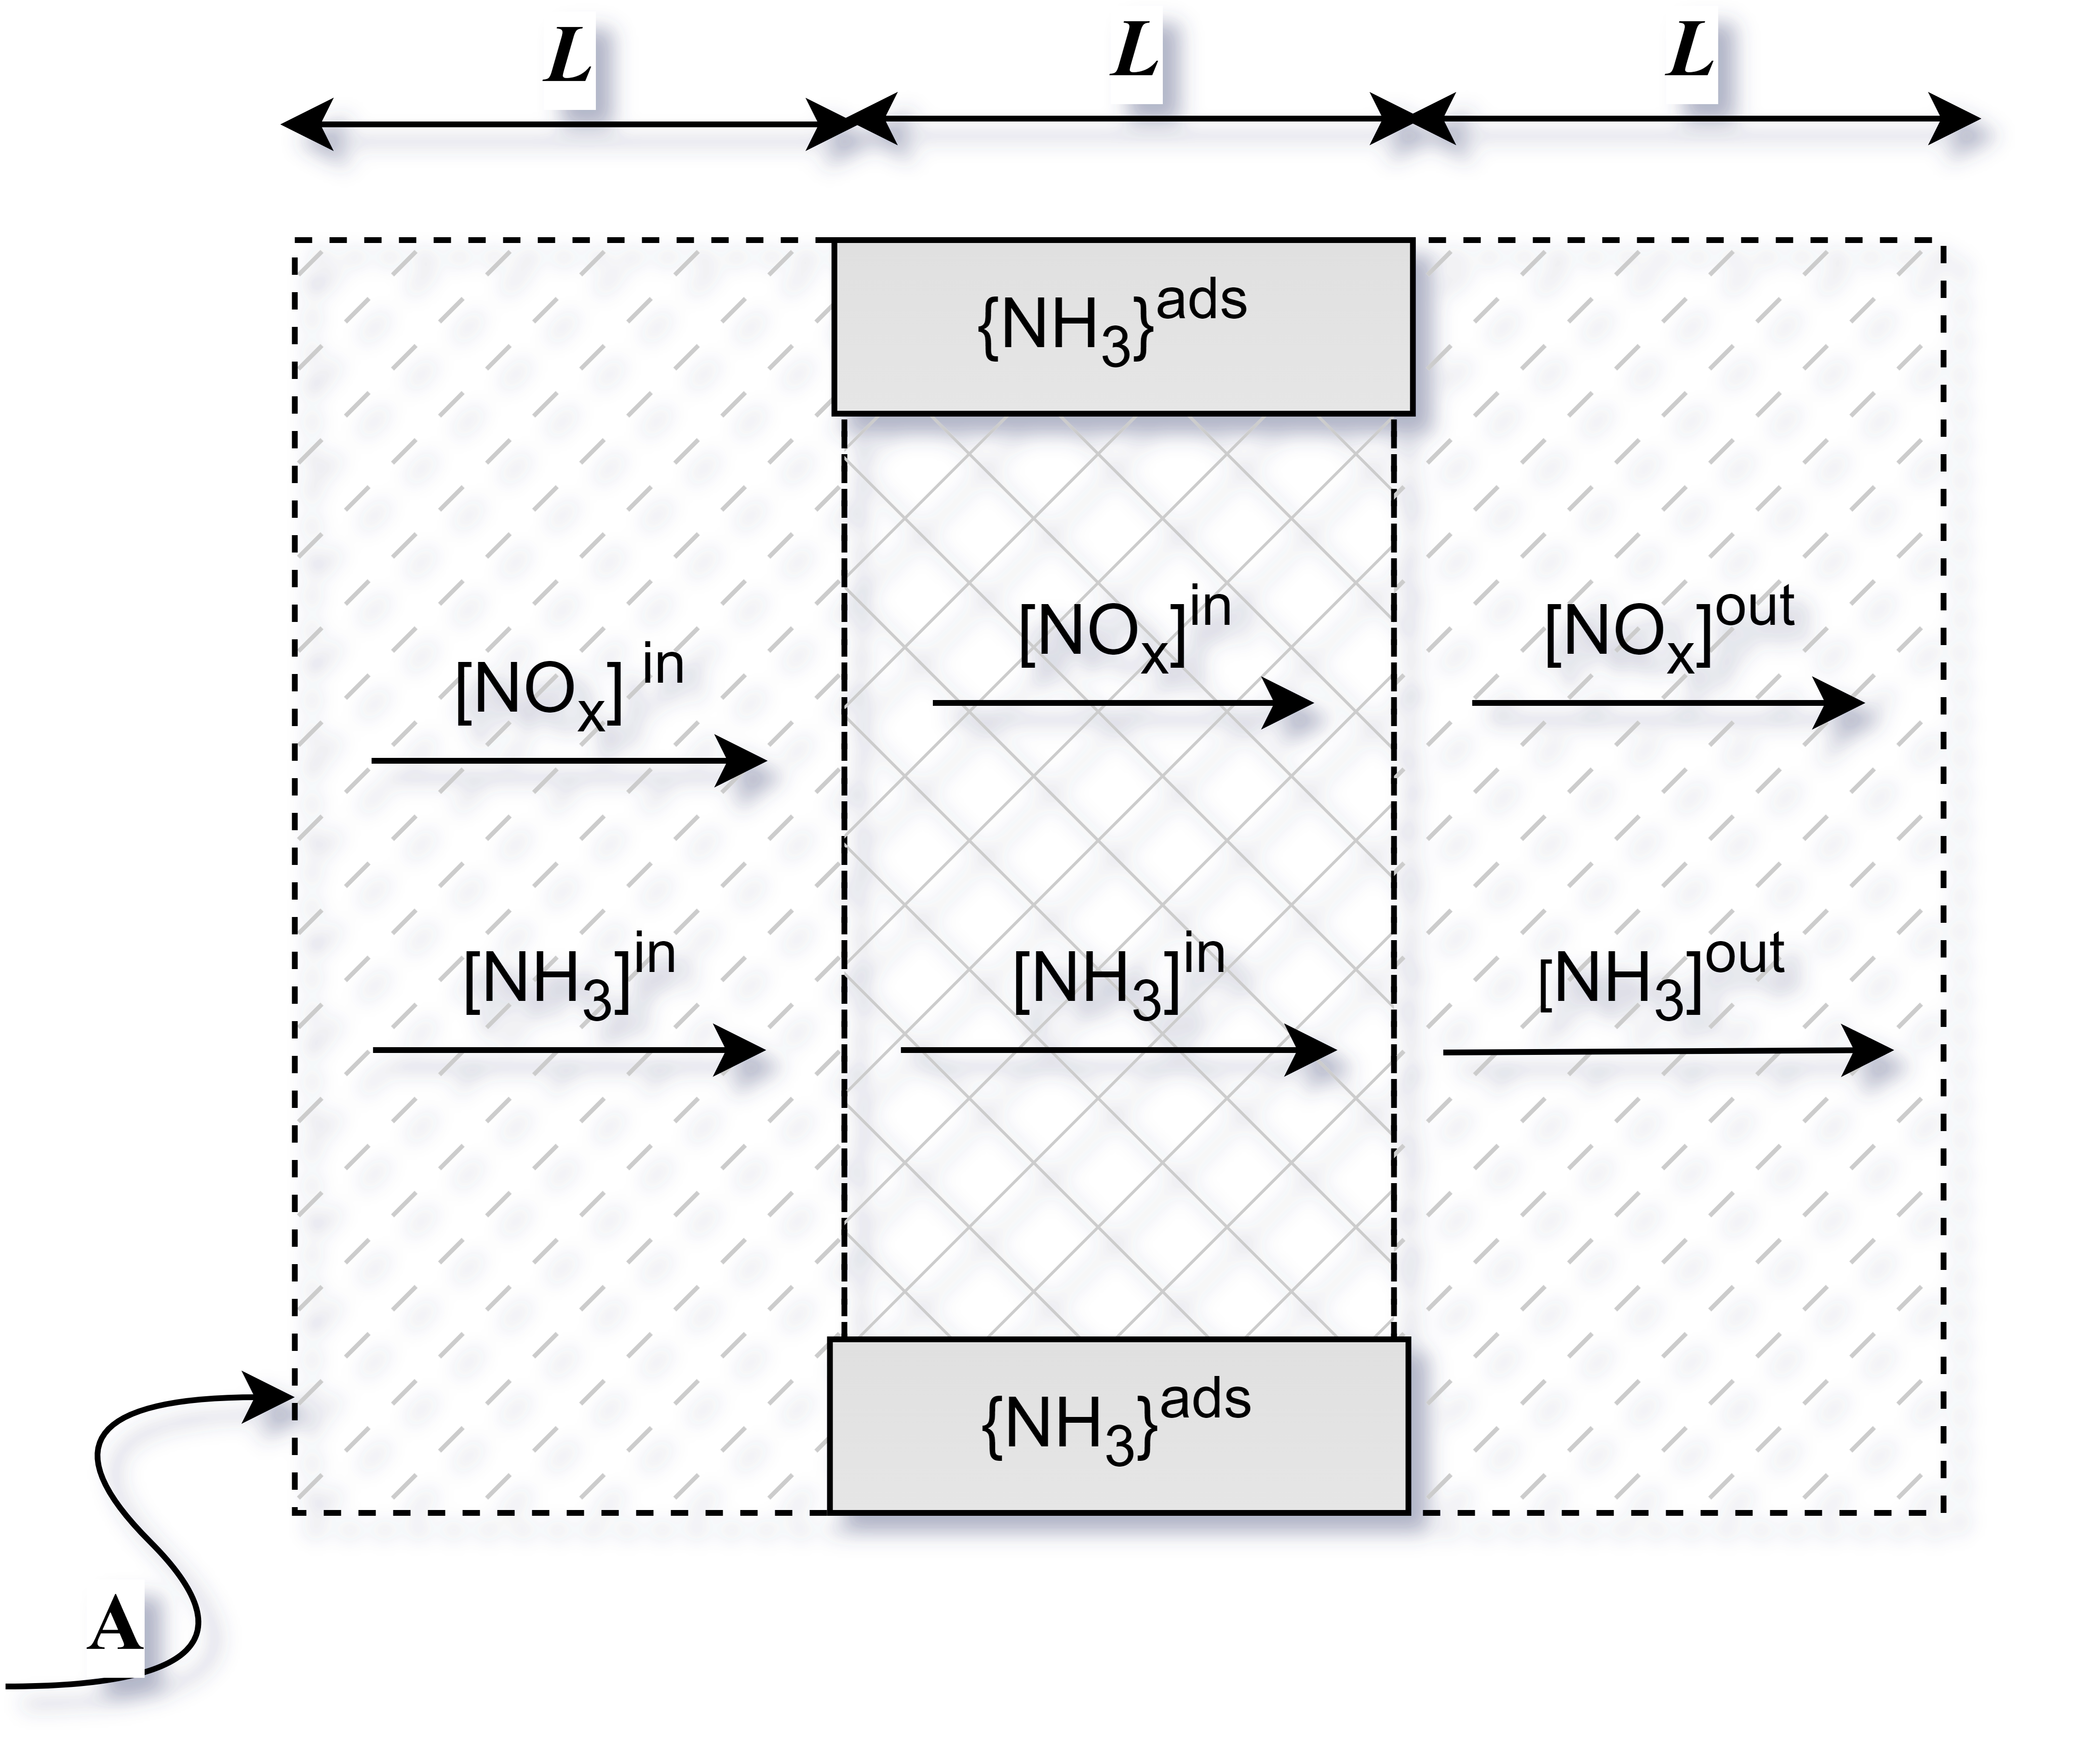
\includegraphics[width = 0.5\textwidth]{\froot/figs/scr_sys/plug_flow_discrete.png}
        \caption{SCR-ASC system abstraction}
\end{figure}
\begin{enumerate}
        \item We have the molar-conservation equations across the control volume within one residence time.
                \begin{multline}
                        \underbrace{\mol{NO_x}^{out} }_{ \con{NO_x}^{out} \tau F_{vol} } (t + (i+1) \tau) =
                                \underbrace{\mol{NO_x}^{in} }_{ \con{NO_x}^{in} \tau F_{vol} } (t + i \tau)
                                + V_{scr} \int_0^{\tau}
                                                \underbrace{\frac{d}{dt} \con{NO_x}^{scr}}_
                                                        {k_{s2v} k_{scr} \con{NO_x}^{in} \con{NH_3}^{ads}}
                                           dt
                        \label{eqn::nox_bal}
                \end{multline}
                \begin{multline}
                       \mol{NH_3}^{ads} (t + (i+1) \tau) =
                                \underbrace{\mol{NH_3}^{ads} }_{A_{scr} \con{NH_3}^{ads}} (t + i \tau)
                                + A_{scr} \int_0^{\tau}
                                               \frac{d}{dt} \con{NH_3}^{ads}
                                               % \underbrace{}_{
                                               %         - \con{NH_3}^{ads}
                                               %                \lrf{
                                               %                k_{ads} \con{NH_3}^{in}
                                               %                + k_{scr} \con{NO_x}^{in}
                                               %                + k_{od}}
                                               %         + \Gamma k_{ads} \con{NH_3}^{in}
                                               %                }
                                                dt
                        \label{eqn::ads_bal}
                \end{multline}
        \item By summing the equations from (\ref{eqn::nox_bal}) for  $i = 0$ to $n-1$, where $n$ is the total number of residence times within one sampling period $(= t_s/\tau)$, we get the relation between the total moles of $NO_x$ that entered, reduced and left the SCR-ASC chamber. Finally, writing the equation in terms of the inlet and outlet concentrations we get the equation relating inlet and outlet concentrations at the end of sampling period as:
                \begin{multline}
                        \underbrace{\con{NO_x}^{out}}_{x_1}(t + t_s) =
                                \underbrace{\con{NO_x}^{in}}_{u_1}(t) + \tau(t) k_{s2v} k_{scr}(t) \con{NO_x}^{in}(t) \underbrace{\lrf{\frac{1}{n} \sum_{i = 0}^{n-1} \con{NH_3}^{ads}(t + i \tau)}}_{\sigma}
                        \label{eqn::nox_avg}
                \end{multline}

        \item The dynamics of $\sigma$, the average surface concentration of adsorbed ammonia on the catalyst for the
                given sampling period, can be obtained by summing the equations from (\ref{eqn::ads_bal}) for $i = 0$ to
                $n-1$ which is the sampling period. This results in a telescopic cancellation of the terms resulting in
                an equation relating the moles in the current sample to the moles in the next sample
                (section-\ref{sec::sigma_deriv}). As the ammonia desorption and ammonia oxidation have the same effect
                ($\sigma$ reduction) on the surface concentration of ammonia in similar fashion, the rate constants can
                be lumped by addition, i.e., $k_{od} = k_{oxi} + k_{dex}$. We have,
                \begin{multline}
                        \sigma(t + t_s) = \sigma(t) - \sigma(t) t_s \lrf{k_{ads}(t) \con{NH_3}^{in}(t)
                                                                                + k_{scr}(t) \con{NO_x}^{in}(t)
                                                                                + k_{od}(t)}
                                                \\
                                                + \Gamma t_s k_{ads}(t) \con{NH_3}^{in}(t)
                        \label{eqn::ads_avg}
                \end{multline}
        \item Finally, using (\ref{eqn::nox_avg}), $\sigma(t+ts), \sigma(t)$ can be eliminated from (\ref{eqn::ads_avg}) for getting a dynamic model for $NO_x$-reduction process which explicitly depends on the measured inputs and states alone.
                \begin{align}
                        \text{Let, }\quad \eta(k) = u_1(k-1) - x_1(k)
                \end{align}
\begin{align*}
        \eta(k+1) =& \eta(k) \lrb{\frac{\tau(k)}{\tau(k-1)}}
                                \lrb{\frac{u_1(k)}{u_1(k-1)}}
                                \lrb{\frac{k_{scr}(k)}{k_{scr}(k-1)}} \\
                &-\eta(k) \lrb{\frac{\tau(k)}{\tau(k-1)}}
                                \lrb{\frac{u_1(k)}{u_1(k-1)}}
                                \lrb{\frac{k_{scr}(k)}{k_{scr}(k-1)}}
                t_s k_{ads}(k-1) \con{NH_3}^{in}(t-1)
                \\
                &-\eta(k) \lrb{\frac{\tau(k)}{\tau(k-1)}}
                                \lrb{\frac{u_1(k)}{u_1(k-1)}}
                                \lrb{\frac{k_{scr}(k)}{k_{scr}(k-1)}}
                t_s k_{scr}(k-1) u_1(k-1)
                \\
                &-\eta(k) \lrb{\frac{\tau(k)}{\tau(k-1)}}
                                \lrb{\frac{u_1(k)}{u_1(k-1)}}
                                \lrb{\frac{k_{scr}(k)}{k_{scr}(k-1)}}
                t_s k_{od}(k-1)
                \\
                &+ t_s k_{s2v} \times \lrf{\Gamma(k-1) \tau(k) u_1(k) \con{NH_3}^{in}(k-1)} \times \lr{k_{scr}(k) k_{ads}(k-1)}
\end{align*}
\begin{equation}
                \label{eqn::disc_NOx}
\end{equation}

\end{enumerate}

The above equation (\ref{eqn::disc_NOx}) is parametrized using the models for the physical properties and
urea-dosing and used for parameter estimation and validation.

Steps, 1, 2 and 3 are discussed in detail in the previous sections. The step-4 derivation is presented below followed by the parametrization.


\subsection{Modelling using average concentration change of $NO_x$ in a sample}
$\eta$ denote the change in concentration from the inlet to outlet in the $NO_x$ in one sample. This is the change in concentration in the exhaust due to the $NO_x$ reduction.
%
\begin{align}
        \eta(k) &= \con{NO_x}^{in}(k-1) - \con{NO_x}^{out}(k) = u_1(k-1) - x_1(k)
\end{align}
%
Thus, rewriting the $NO_x$ process dynamics (\ref{eqn::nox_avg}) interms of $\eta$, we have,
\begin{align}
        \eta(k+1) &= \tau(k) k_{s2v} k_{scr}(k) u_1(k) \sigma(k)\\
        %===
        \implies \sigma(k) &= \frac{\eta(k+1)}{\tau(k) k_{s2v} k_{scr}(k) u_1(k)}
        \label{eqn::sigma_elim}
\end{align}
%
The above equation (\ref{eqn::sigma_elim}) can be used to eliminate the unknown quantity $(\sigma)$ from equation (\ref{eqn::ads_avg}). We have,
\begin{multline}
        \sigma(k+1) = \sigma(k) - \sigma(k) t_s k_{ads}(k) \con{NH_3}^{in}(t)
                        - \sigma(k) t_s k_{scr}(k) u_1(k)
                        - \sigma(k) t_s k_{od}(k)
                        \\ + \Gamma(k) t_s k_ads(k) \con{NH_3}^{in}(k)
\end{multline}
writing the above equation for $\sigma(k)$:
\begin{multline*}
         \sigma(k) = \sigma(k-1)\lrf{1 -  t_s k_{ads}(k-1) \con{NH_3}^{in}(t-1)
                        -  t_s k_{scr}(k-1) u_1(k-1)
                        -  t_s k_{od}(k-1)}
                        \\ + \Gamma(k-1) t_s k_{ads}(k-1) \con{NH_3}^{in}(k-1)
\end{multline*}
Let,
\begin{align}
        \gamma_{proc}(k-1) &= \lrf{1 -  t_s k_{ads}(k-1) \con{NH_3}^{in}(t-1)
                        -  t_s k_{scr}(k-1) u_1(k-1)
                        -  t_s k_{od}(k-1)}
\end{align}
Using equation (\ref{eqn::sigma_elim}),
\begin{multline*}
        \frac{\eta(k+1)}{\tau(k) k_{s2v} k_{scr}(k) u_1(k)}
        = \frac{\eta(k)}{\tau(k-1) k_{s2v} k_{scr}(k-1) u_1(k-1)} \times \gamma_{proc}(k-1)\\
                        \\ + \Gamma(k-1) t_s k_{ads}(k-1) \con{NH_3}^{in}(k-1)
\end{multline*}
Thus, we have the recursive equation for change in concentration due to reduction:
\begin{multline}
        \eta(k+1) = \eta(k) \times \lr{\frac{\tau(k)}{\tau(k-1)}}
                                \times \lr{\frac{u_1(k)}{u_1(k-1)}}
                                \times \lr{\frac{k_{scr}(k)}{k_{scr}(k-1)}}
                                \times \gamma_{proc}(k-1)
                                \\
                        + t_s k_{s2v} \times \lrf{\Gamma(k-1) \tau(k) u_1(k)} \times \lr{k_{scr}(k) k_{ads}(k-1)}
\end{multline}
Explicitly writing the individual terms:
\begin{align*}
        \eta(k+1) =& \eta(k) \lrb{\frac{\tau(k)}{\tau(k-1)}}
                                \lrb{\frac{u_1(k)}{u_1(k-1)}}
                                \lrb{\frac{k_{scr}(k)}{k_{scr}(k-1)}} \\
                &-\eta(k) \lrb{\frac{\tau(k)}{\tau(k-1)}}
                                \lrb{\frac{u_1(k)}{u_1(k-1)}}
                                \lrb{\frac{k_{scr}(k)}{k_{scr}(k-1)}}
                t_s k_{ads}(k-1) \con{NH_3}^{in}(t-1)
                \\
                &-\eta(k) \lrb{\frac{\tau(k)}{\tau(k-1)}}
                                \lrb{\frac{u_1(k)}{u_1(k-1)}}
                                \lrb{\frac{k_{scr}(k)}{k_{scr}(k-1)}}
                t_s k_{scr}(k-1) u_1(k-1)
                \\
                &-\eta(k) \lrb{\frac{\tau(k)}{\tau(k-1)}}
                                \lrb{\frac{u_1(k)}{u_1(k-1)}}
                                \lrb{\frac{k_{scr}(k)}{k_{scr}(k-1)}}
                t_s k_{od}(k-1)
                \\
                &+ t_s k_{s2v} \times \lrf{\Gamma(k-1) \tau(k) u_1(k)} \times \lr{k_{scr}(k) k_{ads}(k-1)}
\end{align*}
The above equation can be simplified using the following two assumptions:
\begin{itemize}
        \item[$A1.$] The temperature doesn't change significantly across contiguous samples, i.e., $T(k-1) \approx T(k)$.
        \begin{align}
                \implies \frac{k_{scr}(k)}{k_{scr}(k-1)} \approx 1
        \end{align}
        \item[$A2.$] The product of rate constants results in a combined rate-constant,
        \begin{align}
                k_{scr}(k) k_{ads}(k-1) &\approx k_{scr}(k-1) k_{ads}(k-1)  = A_{scr}A_{ads} \exp\lrf{\frac{E_{scr}+E_{ads}}{R T(k-1)}} = k_{scr/ads}(k-1)
        \end{align}
\end{itemize}
Incorporating the above assumptions we have the dynamic model for change in concentration due $NO_x$ reduction:
\begin{align*}
         \eta(k+1) =& \eta(k) \lrb{\frac{\tau(k)}{\tau(k-1)}}
                                \lrb{\frac{u_1(k)}{u_1(k-1)}}
                \\
                &-\eta(k) \lrb{\frac{\tau(k)}{\tau(k-1)}}
                                \lrb{\frac{u_1(k)}{u_1(k-1)}}
                t_s k_{ads}(k-1) \con{NH_3}^{in}(t-1)
                \\
                &-\eta(k) \lrb{\frac{\tau(k)}{\tau(k-1)}}
                t_s k_{scr}(k) u_1(k)
                \\
                &-\eta(k) \lrb{\frac{\tau(k)}{\tau(k-1)}}
                                \lrb{\frac{u_1(k)}{u_1(k-1)}}
                t_s k_{od}(k-1)
                \\
                &+ t_s k_{s2v} \times \lrf{\Gamma(k-1) \tau(k) u_1(k)} \times k_{scr/ads}(k-1)
\end{align*}
\begin{equation}
       \label{eqn::nox_govern}
\end{equation}

\subsection{Parametrizing the $\eta$ dynamics}
The equation (\ref{eqn::nox_govern}) can be written in the following structure, with $g_i$'s denoting the corresponding expressions in each of the terms.
\begin{align}
        \eta(k+1) &= \eta(k) \lrf{ g_{\eta} - g_{ads} - g_{od} - g_{scr}} + g_\Gamma
\end{align}
The individual terms, are parametrized based on following relevant set of assumptions:
\begin{itemize}
        \item[$A3.$] The rate constant is linear or (quadratic) for a given operating range of temperature.
        \begin{align}
                k_i &= m_i T + c_i = \underbrace{\bm{T & 1}}_{\pmb \phi^T} \underbrace{\bm{m_i \\ c_i}}_{\pmb \theta_i}
                        = \pmb \phi^{T} \pmb \theta_i
                \qquad \forall \quad T \in \lrb{T_0, T_0 + \Delta T}
                \label{eqn::k_mdl}
        \end{align}
        (or)
        \begin{align}
                k_i &= q_iT^2 + m_i T + c_i = \underbrace{\bm{T^2 & T & 1}}_{\pmb \phi^T} \underbrace{\bm{q_i \\ m_i \\ c_i}}_{\pmb \theta_i}
                        = \pmb \phi^{T} \pmb \theta_i
                \qquad \forall \quad T \in \lrb{T_0, T_0 + \Delta T}
        \end{align}
        %===
        \item[$A4.$] $\Gamma$ is a constant for a given operating range of temperature and only changes with aging.
        \begin{align}
                \Gamma - \text{constant} \quad \forall T \in \lrb{T_0, T_0 + \Delta T}
                \label{eqn::gamma_mdl}
        \end{align}
        %===
        \item[$A5.$] The model for $\con{NH_3}^{in}$ based on urea injection is given by equation (\ref{eqn::urea_inj}), i.e., $\con{NH_3}^{in}$ depends only on the flow-rate and urea injection but not the temperature (as the urea is preheated).
        \begin{align}
                \con{NH_3}^{in}(k) &= \nu_u \times \frac{u_2(k)}{F(k)}
                \label{eqn::urea_mdl}
        \end{align}
        \item[$A6.$] The model for residence time is given by equation (\ref{eqn::res_time}), i.e., the residence time depends only on the flow-rate and effect of change in density (due to change in temperature) is negligable.
        \begin{align}
                \tau(k) &= \frac{V \rho_0}{F(k)} = \frac{\tau_0}{F(k)}
                \label{eqn::residence_time_mdl}
        \end{align}
\end{itemize}

Using the above assumptions, we have the parametrization of individual terms
\begin{enumerate}
\item \begin{align*}
        g_\Gamma &= t_s k_{s2v} \times \lrf{\Gamma(k-1) \tau(k) u_1(k) \con{NH_3}^{in}} \times k_{scr/ads}(k-1)\\
                &= t_s k_{s2v} \Gamma \times \frac{\tau_0}{F(k)} \times u_1 (k) \times \nu_u \frac{u_2(k-1)}{F(k-1)}\times \pmb \phi^T(k-1) \pmb \theta_{scr/ads}
                \qquad \lrb{\because \ref{eqn::gamma_mdl}, \ref{eqn::residence_time_mdl}, \ref{eqn::k_mdl}, \ref{eqn::urea_mdl}}
\end{align*}
\begin{align}
        g_\Gamma &= \lrf{ \frac{u_1(k)}{F(k)} \frac{u_2(k-1)}{F(k-1)} \pmb \phi(k-1) } \times \lrf{ t_s k_{s2v} \nu_u \Gamma \tau_0 \pmb \theta_{scr/ads} }
\end{align}

\item \begin{align*}
        g_{\eta} &= \lrb{\frac{\tau(k)}{\tau(k-1)}}
                                \lrb{\frac{u_1(k)}{u_1(k-1)}}
                = \lrb{\frac{\frac{\tau_0}{F(k)}}{\frac{\tau_0}{F(k-1)}}} \lrb{\frac{u_1(k)}{u_1(k-1)}}
                \qquad \bm{\because \ref{eqn::residence_time_mdl}}
\end{align*}
\begin{align}
        g_{\eta} &= \lrb{\frac{u_1(k)}{F(k)}} \lrb{\frac{F(k-1)}{u_1(k-1)}}
\end{align}

\item \begin{align*}
        g_{ads} &= \lrb{\frac{\tau(k)}{\tau(k-1)}}
                                \lrb{\frac{u_1(k)}{u_1(k-1)}}
                t_s k_{ads}(k-1) \con{NH_3}^{in}(t-1)\\
        % ===
        &=\lrb{\frac{F(k-1)}{F(k)}}\lrb{\frac{u_1(k)}{u_1(k-1)}}
                t_s \times \pmb \phi^T(k-1) \pmb \theta_{ads} \times \nu_u \frac{u_2(t-1)}{F(t-1)}
                \qquad
                \bm{\because \ref{eqn::residence_time_mdl}, \ref{eqn::k_mdl}, \ref{eqn::urea_mdl}}
\end{align*}
\begin{align}
       g_{ads} &=  \lrf{\lrb{\frac{u_1(k)}{F(k)}}\lrb{\frac{u_2(k-1)}{u_1(k-1)}} \pmb \phi^T(k-1) }
                \times \lrf{\nu_u t_s \pmb \theta_{ads}}
\end{align}

\item \begin{align*}
        g_3 &= \lrb{\frac{\tau(k)}{\tau(k-1)}}
                                \lrb{\frac{u_1(k)}{u_1(k-1)}}
                t_s k_{od}(k-1)\\
                &= \lrb{\frac{F(k-1)}{F(k)}}
                                \lrb{\frac{u_1(k)}{u_1(k-1)}}
                t_s \phi^T(k-1) \pmb \theta_{od}
                \qquad \bm{\because \ref{eqn::residence_time_mdl}, \ref{eqn::k_mdl}}
\end{align*}
\begin{align}
        g_3 &= \lrf{ \lrb{\frac{F(k-1)}{F(k)}} \lrb{\frac{u_1(k)}{u_1(k-1)}} \phi^T(k-1) }
                \times \lrf{t_s \pmb \theta_{od}}
\end{align}

\item \begin{align*}
        g_{scr} &= \lrb{\frac{\tau(k)}{\tau(k-1)}}
                t_s k_{scr}(k) u_1(k)\\
                &= \lrb{\frac{F(k-1)}{F(k)}} u_1(k) \pmb \phi^T(k) \pmb \theta_{scr} t_s
                \qquad \bm{\because \ref{eqn::residence_time_mdl}, \ref{eqn::k_mdl}}
\end{align*}
\begin{align}
        g_{scr} &= \lrf{\lrb{\frac{u_1(k)}{F(k)}} F(k-1) \pmb \phi^T(k)}
                \times \lrf{ t_s \pmb \theta_{scr} }
\end{align}

\end{enumerate}

Thus, we have the parametric form of the $NO_x$ reduction dynamics:

\begin{align}
        \eta(k+1) &= \eta(k) \lrb{\frac{u_1(k)}{F(k)}} \lrb{\frac{F(k-1)}{u_1(k-1)}}
                    - \pmb \phi^T_{\eta}(k) \pmb \theta_{\eta}  + \pmb \phi_{\Gamma}^T(k) \pmb \theta_{\Gamma}
        \label{eqn::eta_parm}
\end{align}
where,

\begin{minipage}{0.49\textwidth}
        \begin{align}
                \pmb \phi_{\eta}(k) &= \eta(k) \lrb{\frac{u_1(k)}{F(k)}}
                                \bm{\lrb{\frac{u_2(k-1)}{u_1(k-1)}} \pmb \phi^T(k-1) \\
                                         \lrb{\frac{F(k-1)}{u_1(k-1)}} \pmb \phi^T(k-1)     \\
                                                 F(k-1) \pmb \phi^T(k)
                                                }
        \end{align}
\end{minipage}
\begin{minipage}{0.49\textwidth}
        \begin{align}
        \pmb \theta_{\eta} &= \bm{\nu_u t_s \pmb \theta_{ads}\\
                                        t_s \pmb \theta_{od} \\
                                        t_s \pmb \theta_{scr}}
        \end{align}
\end{minipage}

\begin{minipage}{0.49\textwidth}
        \begin{align}
                \pmb \phi_{\Gamma} (k) &= \lrb{\frac{u_1(k)}{F(k)} } \lrb{ \frac{u_2(k-1)}{F(k-1)}} \pmb \phi(k-1)
        \end{align}
\end{minipage}
\begin{minipage}{0.49\textwidth}
        \begin{align}
                \pmb \theta_{\Gamma} (k) &= \bm{ t_s k_{s2v} \nu_u \Gamma \tau_0 \pmb \theta_{scr/ads} }
        \end{align}
\end{minipage}

\bigskip

Hence, we have the $NO_x$ dynamics:
\begin{align}
        x(k+1) &= u_1(k) - \eta(k) \lrb{\frac{u_1(k)}{F(k)}} \lrb{\frac{F(k-1)}{u_1(k-1)}}
                        + \pmb \phi^T_{\eta}(k) \pmb \theta_{\eta}  - \pmb \phi_{\Gamma}^T(k) \pmb \theta_{\Gamma}
        \label{eqn::nox_sim_mdl}\\
%===
        x(k+1) &= u_1(k) - \lrf{1 - \frac{x_1(k)}{u_1(k-1)}} \lrb{\frac{u_1(k)}{F(k)}} F(k-1)
                        + \pmb \phi^T_{\eta}(k) \pmb \theta_{\eta}  - \pmb \phi_{\Gamma}^T(k) \pmb \theta_{\Gamma}
\end{align}

%==============

$\pmb \phi_\eta$ can be further simplified to avoid the multiplication and division of the same signals that results in noise amplification as follows:

\begin{align}
     \pmb \phi_{\eta}(k)
                        &= \lrb{\frac{u_1(k)}{F(k)}}
                                \bm{\lrb{1 - \frac{x_1(k)}{u_1(k-1)}} u_2(k-1) \pmb \phi^T(k-1) \\
                                     \lrb{1 - \frac{x_1(k)}{u_1(k-1)}}   F(k-1) \pmb \phi^T(k-1)     \\
                                        \eta(k) F(k-1) \pmb \phi^T(k)
                                                }
\end{align}

\subsection{Identification Model}
The parametric model presented previously can be converted to a regression form with minimal noise amplification as follows:
let,
\begin{align}
        \phi_{\eta r}(k) &= \bm{\lrb{1 - \frac{x_1(k)}{u_1(k-1)}} u_2(k-1) \pmb \phi^T(k-1) \\
                                     \lrb{1 - \frac{x_1(k)}{u_1(k-1)}}   F(k-1) \pmb \phi^T(k-1)     \\
                                        \eta(k) F(k-1) \pmb \phi^T(k)
                                                }\\
        \phi_{\Gamma r}(k) &= \lrb{ \frac{u_2(k-1)}{F(k-1)}} \pmb \phi(k-1)
\end{align}
Thus, rewriting equation (\ref{eqn::eta_parm}):
\begin{align*}
        \lrb{\frac{F(k)}{u_1(k)}} \eta(k+1) &= \eta(k) \lrb{\frac{F(k-1)}{u_1(k-1)}}
                    - \pmb \phi^T_{\eta r}(k) \pmb \theta_{\eta}  + \pmb \phi_{\Gamma r}^T(k) \pmb \theta_{\Gamma}
\end{align*}
Let,
\begin{align}
        y_{NO_x}(k) &= \lrb{\frac{F(k)}{u_1(k)}} \eta(k+1) - \eta(k) \lrb{\frac{F(k-1)}{u_1(k-1)}} \\
        %====
        \pmb \phi_{NO_x}(k) &= \bm{- \pmb \phi_{\eta r}(k) \\
                          \pmb \phi_{\Gamma r}(k)}
                        = \bm{\lrb{\frac{x_1(k)}{u_1(k-1)} - 1} u_2(k-1) \pmb \phi^T(k-1) \\
                                     \lrb{\frac{x_1(k)}{u_1(k-1)} - 1}   F(k-1) \pmb \phi^T(k-1)     \\
                                        - \eta(k) F(k-1) \pmb \phi^T(k) \\
                                                \lrb{ \frac{u_2(k-1)}{F(k-1)}} \pmb \phi(k-1)}
        \label{eqn::phi_NOx}\\
        %===
        \pmb \theta_{NO_x} &= \bm{\pmb \theta_{\eta} \\
                                  \pmb \theta_{\Gamma}}
                            = \bm{\nu_u t_s \pmb \theta_{ads}\\
                                        t_s \pmb \theta_{od} \\
                                        t_s \pmb \theta_{scr} \\
                                        t_s k_{s2v} \nu_u \Gamma \tau_0 \pmb \theta_{scr/ads}}
\end{align}
Thus, we have the regression model,
\begin{align}
        y_{NO_x}(k) &= \pmb \phi_{NO_x}^T \pmb \theta_{NO_x}
        \label{eqn::ident_form}
\end{align}

\subsection{Physical Interpretation of the Model}
We have the tailpipe $NO_x$ dynamics (\ref{eqn::nox_sim_mdl}):
\begin{align}
        x(k+1) &= u_1(k) - \eta(k) \lrb{\frac{u_1(k)}{F(k)}} \lrb{\frac{F(k-1)}{u_1(k-1)}}
                        + \lrb{\frac{u_1(k)}{F(k)}} \pmb \phi_{NO_x}(k) \pmb \theta_{NO_x}
        \label{eqn::NOx_simulation}
\end{align}
\begin{multline}
        \implies \underbrace{x(k+1)}_{\bm{\text{tailpipe (outlet) $NO_x$}\\ \text{at next time step}}}
        % ===
        = \underbrace{u_1(k)}_{\bm{\text{engine-out (inlet) concentration}\\
                                   \text{at current time step}}}
                - \underbrace{ \eta(k) \lrb{\frac{u_1(k)}{F(k)}} \lrb{\frac{F(k-1)}{u_1(k-1)}}}
                                _{\bm{\text{$NO_x$ reduction }\\
                                        \text{from previous step}\\
                                        \text{corrected for current flow-rate}}}
                                \\+ \underbrace{
                                \bm{\lrb{1 - \frac{x_1(k)}{u_1(k-1)}} u_2(k-1) \pmb \phi^T(k-1) \\
                                     \lrb{1 - \frac{x_1(k)}{u_1(k-1)}}   F(k-1) \pmb \phi^T(k-1)     \\
                                         \eta(k) F(k-1) \pmb \phi^T(k) \\
                                         - \lrb{ \frac{u_2(k-1)}{F(k-1)}} \pmb \phi(k-1)}
                                \bm{\nu_u t_s \pmb \theta_{ads}\\
                                        t_s \pmb \theta_{od} \\
                                        t_s \pmb \theta_{scr} \\
                                        t_s k_{s2v} \nu_u \Gamma \tau_0 \pmb \theta_{scr/ads}}
                                }_{
                                        \bm{\text{change in $NO_x$ reduction due to} \\
                                                \text{change in adsorbed ammonia from} \\
                                                \text{oxidation, urea-injection and}\\
                                                \text{change in void concentration}
                                        }
                                }
\end{multline}

The model predicts the tailpipe $NO_x$ from the engine-out $NO_x$ and the previous change in concentration due to
reduction. The change in adsorbed ammonia concentration due to oxidation, SCR reaction and change in void concentration
is implicitly considered.

\subsection{Switched model for wider temperature ranges}

The only restrictive assumption in the derivation of the above model is related to the temperature range of operation.
The linear temperature dependence of rate constants and independence of density (thereby residence time) and void
fraction of the catalyst are valid for a narrow range of temperatures. The other nonlinear effects due to flow-rate and
urea injection are captured in the model. Introducing more complex temperature models for the physical quantities would
lead to parametric models that are not linear (in parameters) and identifiable. Thus, a hybrid model is proposed where
the model structure remains the same while the parameters switch depending on the temperature.

\begin{multline}
        x(k+1) = u_1(k) - \eta(k) \lrb{\frac{u_1(k)}{F(k)}} \lrb{\frac{F(k-1)}{u_1(k-1)}}
                        + \lrb{\frac{u_1(k)}{F(k)}} \pmb \phi^{T}_{NO_x}(k) \pmb \theta^i_{NO_x}
        \\
        T(k), T(k-1) \in \lrb{T_i-\Delta T, T_i + \Delta T}
\end{multline}

Thus, the system switches between models when the current temperature is beyond the $\pm \Delta T$ range of the model.
Experience from the linearized model identification suggests that $\Delta T \approx 25 \, ^0C$ would account for
the changes in system parameters due to drastic changes in temperature.

As the model doesn't have explicit dependence on the unmeasured initial conditions, the parameters for the switched system can be identified by partitioning the data based on the temperature.

\subsubsection{Temperature partitioning}

The temperature partitions work if we have enough data for satisfying PE condition in each of the partitions. From the actual temperature ranges of the test-cell data we get the following narrow partitioning to maximize the length of data available in each of the partitions, which can be used for the linear temperature model:

\begin{figure}[H]
        \centering
        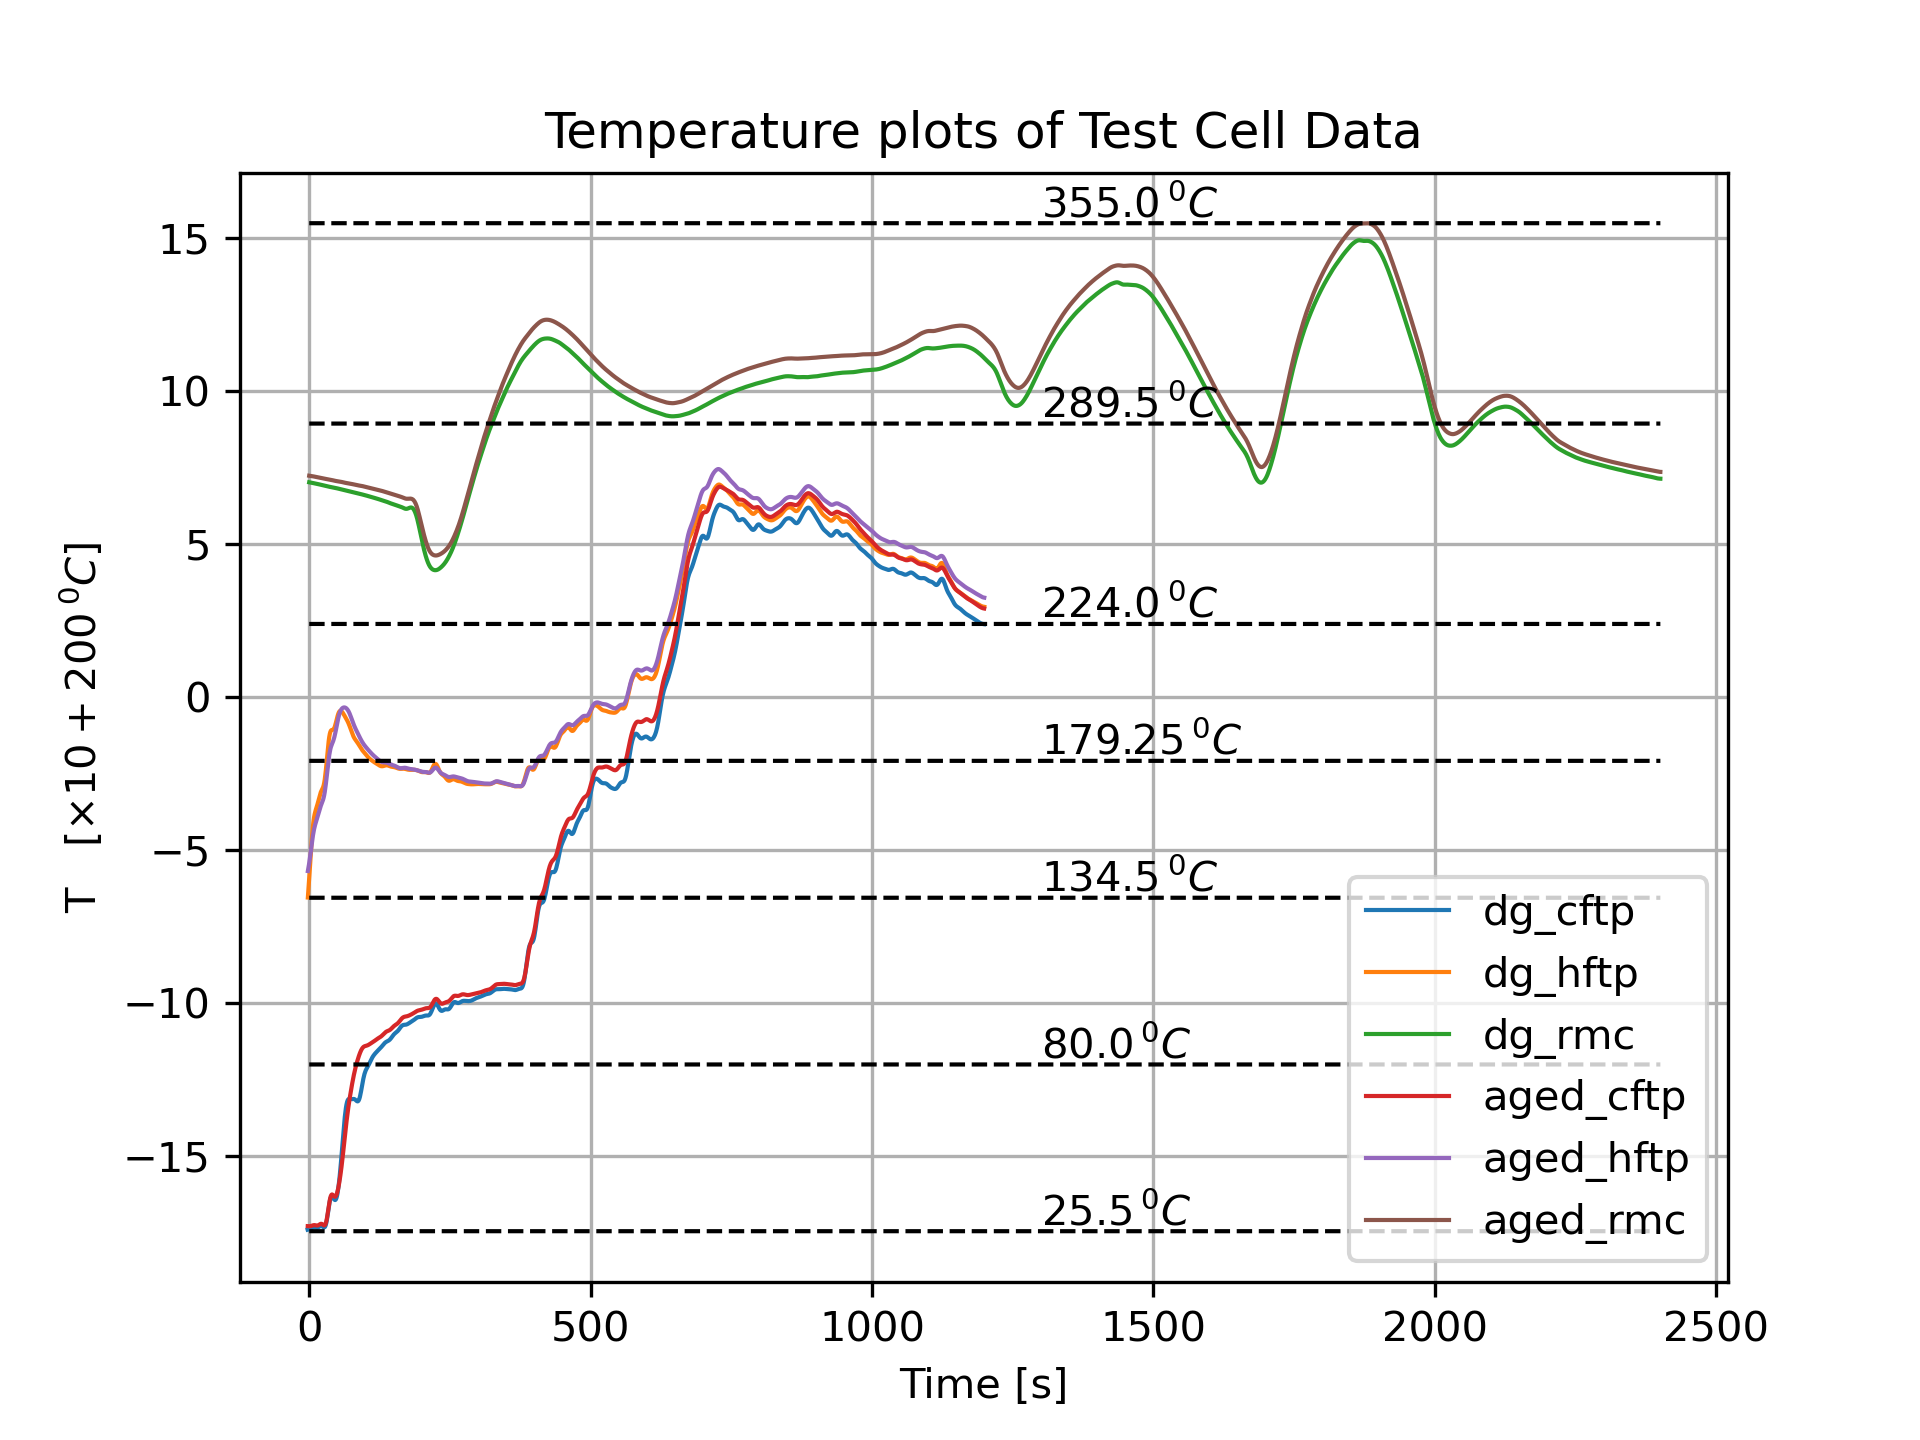
\includegraphics[width = 0.5\textwidth]{\froot/figs/12_figs/hybrid_ssd_T.png}
        \caption{Temperature partitioning for the hybrid model in test-cell case}
\end{figure}

The partitions can be further narrowed if the prediction error is not within the satisfactory range. Alternately, a
wider partition, namely high and low temperature zones, seems to be enough to consistently model the test-cell data when
using a combination of linear and quadratic temperature models for rate-constants. This partitioning has a
high-temperature region where all of RMC test and hot-FTP test lie and a low-temperature region where only a part of the
cold-FTP test lies. This partitioning worked the best for the saturated model parameter estimation with quadratic
temperature model for $\Gamma k_{ads/scr}$ parametrization. The desaturated model uses the same model with linear
temperature model for $k_i, i=ads, scr, od$ parametrization and a quadratic for $\Gamma k_{ads/scr}$ parametrization
similar to the saturated system. Further analysis using AVL cruise data is required to obtain the optimal partitioning
and order for temperature models of the rate-constants.

\begin{figure}[H]
        \centering
        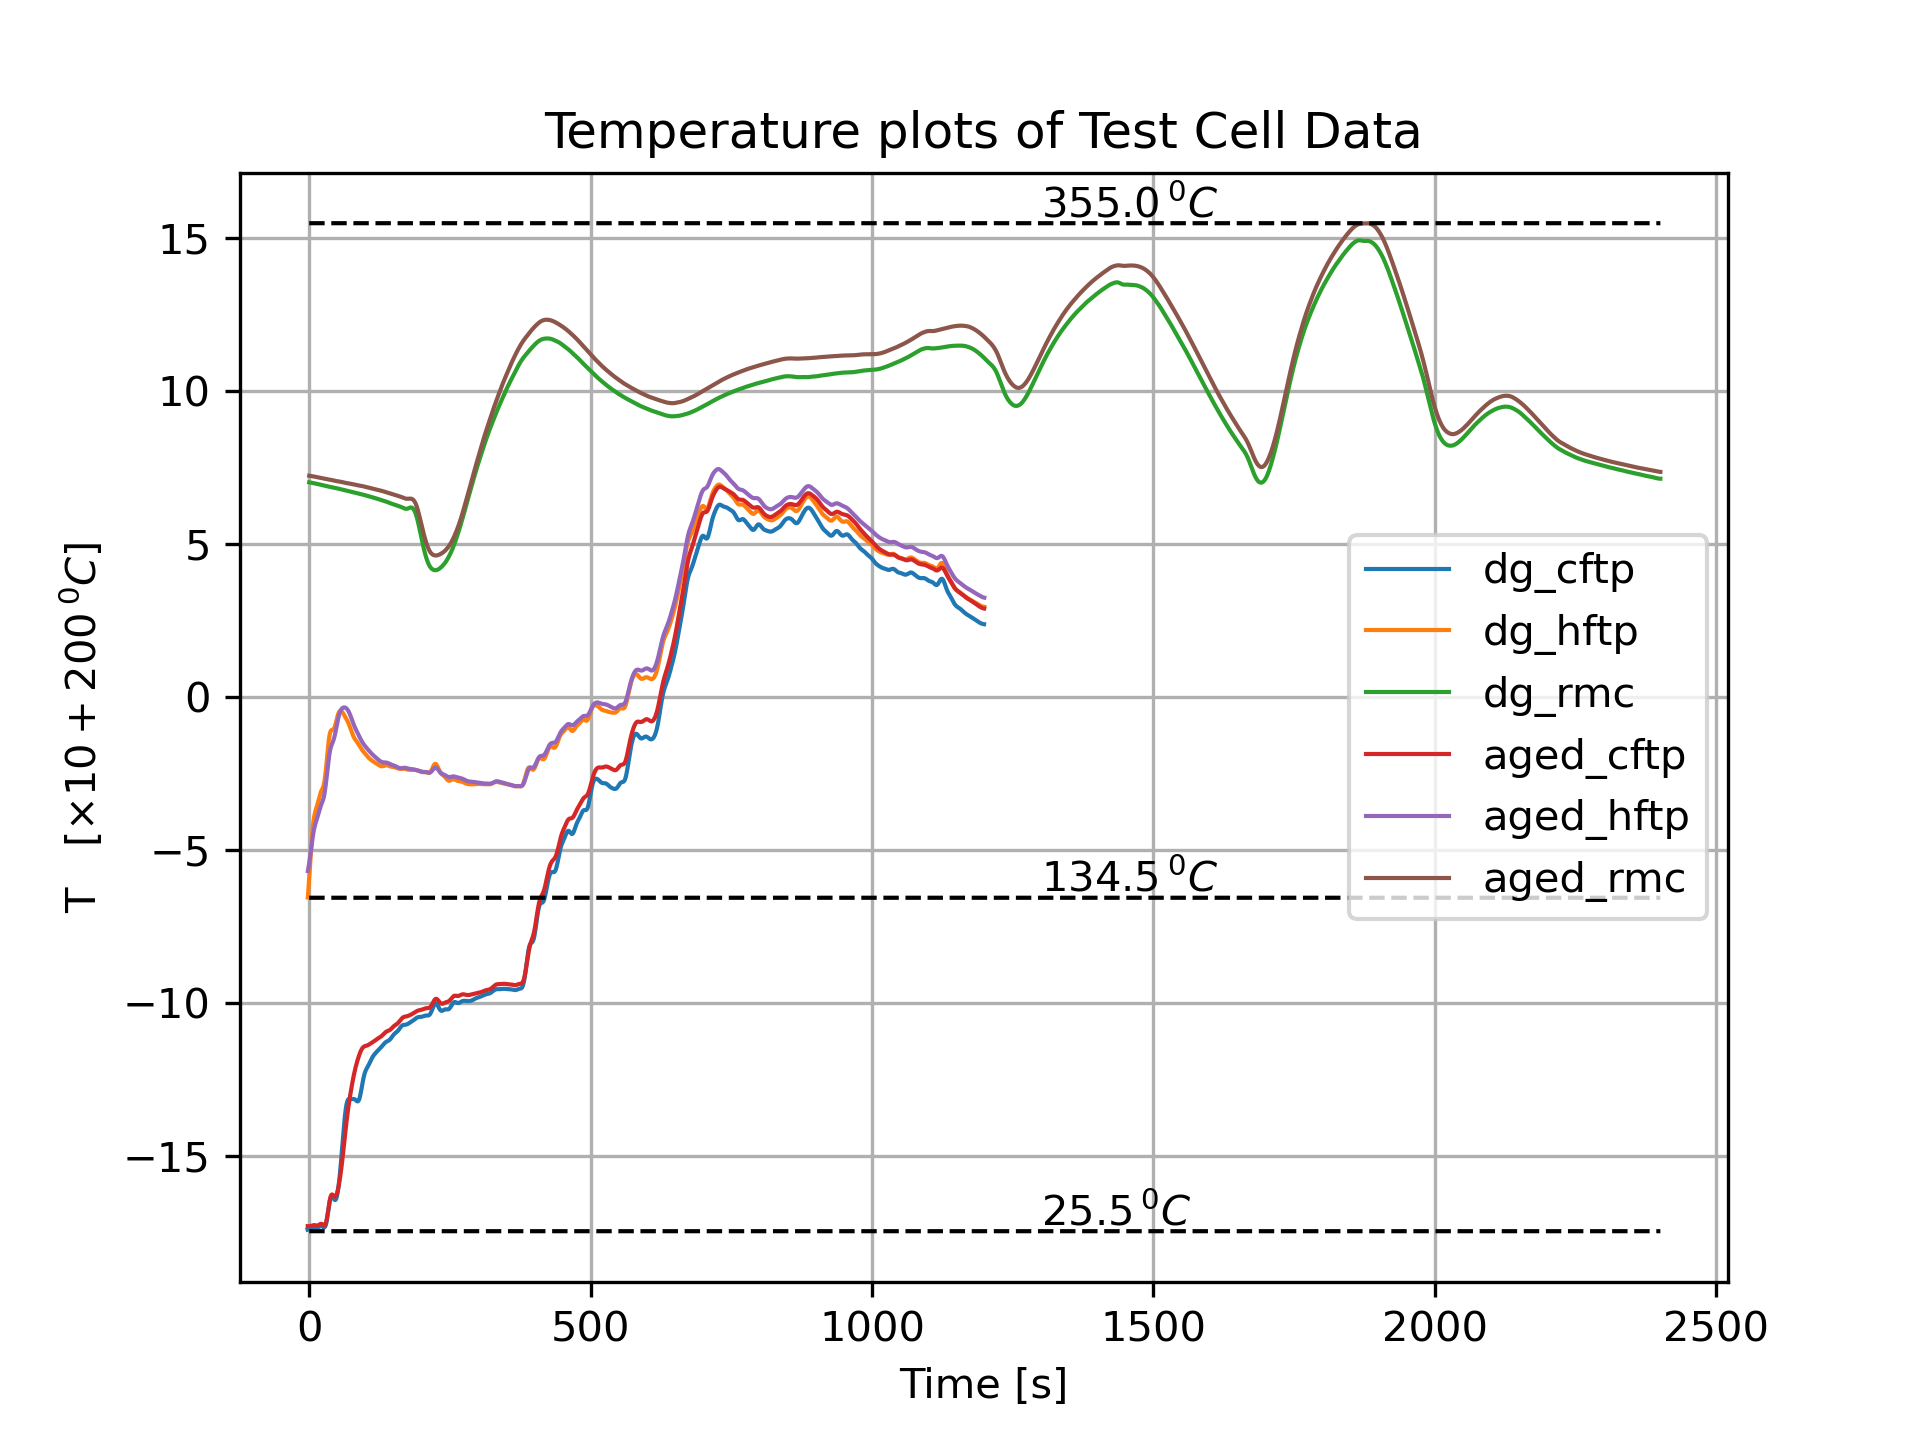
\includegraphics[width = 0.5\textwidth]{\froot/figs/12_figs/hybrid_ssd_hl_T.png}
        \caption{2-zone temperature partitioning for the hybrid model in test-cell case}
\end{figure}

